\chapter{Grafi}
Moltissimi problemi possono essere visti come problemi sui \emph{grafi} e
sebbene questi abbiano forma astratta, le loro soluzioni trovano applicazioni
negli ambiti più disparati.

Abbiamo già dato una prima definizione generica di \hyperref[def:30]{\emph{grafo}},
ma adesso andremo ad estenderla introducendo una serie di concetti che saranno
necessari per affrontare proficuamente questo capitolo.

\section{Introduzione}
Diamo le seguenti definizioni.

\begin{definition}[Grafo orientato]
    Un grafo orientato è una coppia $G=(V,E)$ dove $V$ è l'insieme dei vertici,
    o dei nodi, del grafo ed $E$ è un insieme di coppie ordinate di nodi $(u,v)$
    per $u,v\in V$ dette archi, o lati.
\end{definition}
\begin{figure}[ht]
    \centering
    \resizebox*{0.44\textwidth}{!}{
      $\begin{array}[c]{rcl}
        V & = & \{\,a,b,c,d,e,f\,\}\\
        E & = & \{\,(a,b),(a,d),(d,a),\\
          &   &  \ \ (b,c),(d,c),(d,e),\\
          &   &  \ \ (e,c)\,\}
      \end{array}$
    }\hfill
    \resizebox*{0.52\textwidth}{!}{
      \begin{graph}
        \node[main] (0) {$a$};
        \node[main] (1) [above right of=0, xshift=30] {$b$};
        \node[main] (2) [below right of=0, xshift=30] {$d$};
        \node[main] (3) [right of=1, xshift=30] {$c$};
        \node[main] (4) [right of=2, xshift=30] {$e$};
        \node[main] (5) [below right of=3] {$f$};
    
        \draw[->] (0) -- (1);
        \draw[->] (0) edge[bend left=20] (2);
        \draw[<-] (0) edge[bend right=20] (2);
        \draw[->] (1) -- (3);
        \draw[->] (2) -- (3);
        \draw[->] (2) -- (4);
        \draw[->] (4) -- (3);
      \end{graph}
    }
    \caption{\emph{Grafo orientato}}
\end{figure}

\begin{definition}[Grafo non orientato]
    Un grafo non orientato è una coppia $G=(V,E)$ dove $V$ è l'insieme dei vertici,
    o dei nodi, del grafo ed $E$ è un insieme di coppie non ordinate di nodi $(u,v)$
    per $u,v\in V$ dette archi, o lati.
\end{definition}\newpage
\begin{figure}[ht]
    \centering
    \resizebox*{0.44\textwidth}{!}{
      $\begin{array}[c]{rcl}
        V & = & \{\,a,b,c,d,e,f\,\}\\
        E & = & \{\,(a,b),(a,d),(b,c),\\
          &   &  \ \ (d,c),(d,e),(e,c)\,\}
      \end{array}$
    }\hfill
    \resizebox*{0.52\textwidth}{!}{
      \begin{graph}
        \node[main] (0) {$a$};
        \node[main] (1) [above right of=0, xshift=30] {$b$};
        \node[main] (2) [below right of=0, xshift=30] {$d$};
        \node[main] (3) [right of=1, xshift=30] {$c$};
        \node[main] (4) [right of=2, xshift=30] {$e$};
        \node[main] (5) [below right of=3] {$f$};
    
        \draw (0) -- (1);
        \draw (0) -- (2);
        \draw (1) -- (3);
        \draw (2) -- (3);
        \draw (2) -- (4);
        \draw (4) -- (3);
      \end{graph}
    }
    \caption{\emph{Grafo non orientato}}
\end{figure}

\begin{note}
    I \emph{grafi orientati} e \emph{non orientati} sono anche detti,
    rispettivamente, \emph{directed} e \emph{undirected}.
\end{note}\noindent
In un \emph{grafo orientato} un \emph{vertice} $v$ è detto \emph{adiacente} a $u$
se esiste un \emph{arco} $(u,v)$ e, quell'arco, è detto \emph{incidente} da
$u$ in $v$. Ovviamente, in un \emph{grafo non orientato} la nozione di
\emph{adiacenza} è simmetrica.
\begin{eg}[Adiacenza e incidenza]
    Nel seguente grafo orientato, per la parte evidenziata, valgono le seguenti
    relazioni di adiacenza e incidenza.\\
    \begin{minipage}{0.48\textwidth}
        \centering
        \begin{graph}
            \node[main, line width=1.3pt] (0) {$a$};
            \node[main, line width=1.3pt] (1) [above right of=0, xshift=30] {$b$};
            \node[main, line width=1.3pt] (2) [below right of=0, xshift=30] {$d$};
            \node[main] (3) [right of=1, xshift=30] {$c$};
            \node[main] (4) [right of=2, xshift=30] {$e$};
            \node[main] (5) [below right of=3] {$f$};
        
            \draw[->, line width=1.3pt] (0) -- (1);
            \draw[->] (0) edge[bend left=20, line width=1.3pt] (2);
            \draw[<-] (0) edge[bend right=20, line width=1.3pt] (2);
            \draw[->] (1) -- (3);
            \draw[->] (2) -- (3);
            \draw[->] (2) -- (4);
            \draw[->] (4) -- (3);
        \end{graph}
    \end{minipage}
    \hfill
    \begin{minipage}{0.48\textwidth}
        \par\noindent
        \begin{itemize}
            \item $(a,b)$ è incidente da $a$ a $b$;
            \item $(a,d)$ è incidente da $a$ a $d$;
            \item $(d,a)$ è incidente da $d$ ad $a$;
            \item $b$ è adiacente ad $a$;
            \item $d$ è adiacente ad $a$;
            \item $a$ è adiacente a $d$;
        \end{itemize}
    \end{minipage}
\end{eg}

\subsection{Dimensioni dei grafi}
\begin{definition}[Numero di nodi e di archi]
    Dato un grafo $G=(V,E)$ il numero di nodi e il numero di archi corrispondono,
    rispettivamente, alla cardinalità degli insiemi $V$ ed $E$.
\end{definition}
\begin{note}
    Di seguito, salvo diverse indicazioni, indicheremo con $n$ il numero di
    \emph{nodi} e con $m$ il numero di \emph{archi}, cioè $n=|V|$ ed $m=|E|$.
\end{note}

\begin{definition}[Numero massimo di archi in un grafo orientato]
    Dato un grafo orientato vale la seguente relazione sul numero di
    archi:
    \[m\leq n(n-1)\]
\end{definition}
\begin{definition}[Numero massimo di archi in un grafo non orientato]
    Dato un grafo non orientato vale la seguente relazione sul numero
    di archi:
    \[m\leq\frac{n(n-1)}{2}\]
\end{definition}
\begin{note}
    In entrambi i casi possiamo affermare che il numero di \emph{archi} è $O(n^2)$.
\end{note}
\begin{note}
    Per gli algoritmi che operano sui \emph{grafi} la \emph{complessità} è espressa
    sia in termine di $n$ che $m$ e quindi considereremo \emph{lineare} un
    algoritmo con \emph{complessità} $O(n+m)$.
\end{note}

\subsection{Casi speciali}
\begin{definition}[Grafo completo]
    Un grafo con un arco tra tutte le coppie di nodi è detto completo.
\end{definition}
\begin{definition}[Grafi sparsi e densi]
    Un grafo con \q{pochi archi} è detto essere sparso, mentre uno con \q{tanti
    archi}, denso.
\end{definition}
\begin{note}
    La definizione di \emph{grafi sparsi} e \emph{densi} non è formale, ma
    tendenzialmente un \emph{grafo} con $m=O(n)$ o $O(n\log n)$ è considerato
    \emph{sparso}. Sono invece considerati \emph{densi} i \emph{grafi} con
    $m=\Omega(n^2)$.
\end{note}

\bigskip\noindent
Possiamo definire gli \emph{alberi} in funzione dei \emph{grafi}.
\begin{definition}[Albero libero]
    Un grafo con $m=n-1$ è detto albero libero.
\end{definition}
\begin{definition}[Albero radicato (visto come grafo)]
    Un grafo connesso con $m=n-1$ archi nel quale uno dei nodi è stato designato
    come radice è detto albero radicato.
\end{definition}
\begin{definition}[Foresta]
    Un insieme di alberi è detto foresta.
\end{definition}

\subsection{Cammini e gradi dei nodi}
\begin{definition}[Cammino]
    In un grafo $G=(V,E)$, una sequenza di $k+1$ nodi $u_0,\,u_1,\,\dots,\,u_k$ è
    definita essere un cammino di lunghezza $k$, se è tale per cui l'arco
    $(u_i,u_{i+1})\in E$ $\forall\,0\leq i\leq k-1$.
\end{definition}

\begin{eg}[Cammino]
\begin{minipage}{0.45\textwidth}
    \vspace{0.2cm}
    \hspace{0.2cm}
    \begin{graph}
        \node[main] (0) {$a$};
        \node[main] (1) [above right of=0, xshift=30] {$b$};
        \node[main] (2) [below right of=0, xshift=30] {$d$};
        \node[main] (3) [right of=1, xshift=30] {$c$};
        \node[main] (4) [right of=2, xshift=30] {$e$};
    
        \draw[line width=1.3pt] (0) -- (1);
        \draw[line width=1.3pt] (1) -- (3);
        \draw (2) -- (3);
        \draw[line width=1.3pt] (2) -- (4);
        \draw[line width=1.3pt] (4) -- (3);
    \end{graph}
\end{minipage}
\hfill
\begin{minipage}{0.53\textwidth}
    La sequenza di nodi $a,b,c,e,d$ è un cammino di lunghezza $4$.

    \paragraph{NB}
    In questo caso il cammino è anche detto semplice perché tutti i nodi
    che lo compongono sono distinti.
\end{minipage}
\end{eg}

\begin{definition}[Grado di un nodo in un grafo orientato]
    In un grafo orientato si definisce grado entrante di un nodo il numero di
    archi incidenti su di esso, mentre il grado uscente è definito come il numero
    di archi incidenti da esso.
\end{definition}
\begin{definition}[Grado di un nodo in un grafo non orientato]
    In un grafo non orientato il grado di un nodo è definito come il numero di
    archi incidenti su di esso.
\end{definition}

\begin{figure}[ht]
    \centering
    \subfloat[\emph{Grafo orientato}]
    {
        \resizebox*{0.48\textwidth}{!}{
            \begin{graph}
                \node[main, label={$\begin{array}{rr}
                  \emph{in} & 1\\
                  \emph{out} & 2
                \end{array}$}] (0) {$a$};
                \node[main, label={$\begin{array}{rr}
                  \emph{in} & 1\\
                  \emph{out} & 1
                \end{array}$}] (1) [above right of=0, xshift=30] {$b$};
                \node[main, label=below:{$\begin{array}{rr}
                  \emph{in} & 1\\
                  \emph{out} & 3
                \end{array}$}] (2) [below right of=0, xshift=30] {$d$};
                \node[main, label={$\begin{array}{rr}
                  \emph{in} & 3\\
                  \emph{out} & 0
                \end{array}$}] (3) [right of=1, xshift=30] {$c$};
                \node[main, label=below:{$\begin{array}{rr}
                  \emph{in} & 1\\
                  \emph{out} & 1
                \end{array}$}] (4) [right of=2, xshift=30] {$e$};
                \node[main, label={$\begin{array}{rr}
                  \emph{in} & 0\\
                  \emph{out} & 0
                \end{array}$}] (5) [below right of=3] {$f$};
            
                \draw[->] (0) -- (1);
                \draw[->] (0) edge[bend left=20] (2);
                \draw[<-] (0) edge[bend right=20] (2);
                \draw[->] (1) -- (3);
                \draw[->] (2) -- (3);
                \draw[->] (2) -- (4);
                \draw[->] (4) -- (3);
              \end{graph}
        }
    }
    \hfill
    \subfloat[\emph{Grafo non orientato}]
    {\resizebox*{0.48\textwidth}{!}{
        \begin{graph}
            \node[main, label={$2$}] (0) {$a$};
            \node[main, label={$2$}] (1) [above right of=0, xshift=30] {$b$};
            \node[main, label=below:{$3$}] (2) [below right of=0, xshift=30] {$d$};
            \node[main, label={$3$}] (3) [right of=1, xshift=30] {$c$};
            \node[main, label=below:{$2$}] (4) [right of=2, xshift=30] {$e$};
            \node[main, label={$0$}] (5) [below right of=3] {$f$};
        
            \draw (0) -- (1);
            \draw (0) -- (2);
            \draw (1) -- (3);
            \draw (2) -- (3);
            \draw (2) -- (4);
            \draw (4) -- (3);
          \end{graph}
    }}
    \caption{\emph{Grado} dei \emph{nodi} nei \emph{grafi orientati} e \emph{non orientati}}
\end{figure}

\subsection{Specifica}
\begin{code}{Grafo}
    \com{Crea un nuovo \emph{grafo}}
    \bc{GRAPH} Graph()
    \nl\com{Restituisce l'insieme di tutti i \emph{vertici}}
    \bc{SET} V()
    \nl\com{Restituisce il numero di \emph{nodi}}
    \bc{int} size()
    \nl\com{Restituisce l'insieme dei \emph{nodi adiacenti} ad $u$}
    \bc{SET} adj(\bc{NODE} u)
    \nl\com{Aggiunge un \emph{nodo} $u$ al \emph{grafo}}
    insertNode(\bc{NODE} u)
    \nl\com{Aggiunge l'\emph{arco} $(u,v)$ al \emph{grafo}}
    insertEdge(\bc{NODE} u, \bc{NODE} v)
    \nl\com{Rimuove il \emph{nodo} $u$ dal \emph{grafo}}
    removeNode(\bc{NODE} u)
    \nl\com{Rimuove l'\emph{arco} $(u,v)$ dal \emph{grafo}}
    removeEdge(\bc{NODE} u, \bc{NODE} v)
\end{code}

\subsection{Memorizzare un grafo}
Per la memorizzazione dei \emph{grafi} esistono due approcci: \emph{matrici di
adiacenza} e \emph{liste di adiacenza}.

\paragraph{Memorizzazione di un grafo orientato}
L'approccio con \emph{matrice di adiacenza} prevede che venga realizzata una
matrice $n\times n$ tale che:
\[m_{u,v}=\begin{cases}
    1 & \text{se } (u,v)\in E\\
    0 & \text{se } (u,v)\notin E
\end{cases}\]
Quindi, il \emph{grafo} viene rappresentato tramite una matrice di
valori binari nella quale la cella che si trova nell'$u$-esima riga e $v$-esima
colonna è 1 se e solo se esiste un \emph{arco} da $u$ a $v$.

D'altra parte, le \emph{liste di adiacenza} sfruttano il concetto di
\emph{adiacenza} espresso nelle specifiche dalla funzione \texttt{adj}. Vale
infatti, la seguente definizione matematica di \texttt{adj} e quindi di
\emph{adiacenza}:
\[G.adj(u)=\{v\,|\,(u,v)\in E\}\]
Quindi, nell'approccio basato su \emph{liste}, viene realizzata una \emph{lista}
contenente tutti i \emph{vertici} del \emph{grafo}. Ogni \emph{nodo} della
\emph{lista} poi, a cascata, contiene un riferimento ad un uno dei \emph{vertici}
che nel \emph{grafo} sono \emph{adiacenti} al \emph{vertice} associato a quel
\emph{nodo} della \emph{lista}.

\begin{figure}[h!]
    \centering
    \subfloat[\emph{Grafo orientato}]
    {
        \begin{graph}
            \node[main] (0) {$0$};
            \node[main] (1) [right of=0, xshift=30] {$1$};
            \node[main] (2) [below of=0, yshift=-30] {$3$};
            \node[main] (3) [right of=1, xshift=30] {$2$};
            \node[main] (4) [right of=2, xshift=30] {$4$};
            \node[main] (5) [below of=3, yshift=-30] {$5$};
        
            \draw[->] (0) -- (1);
            \draw[<-] (0) edge[bend left=20] (2);
            \draw[->] (0) edge[bend right=20] (2);
            \draw[->] (1) -- (3);
            \draw[->] (2) -- (3);
            \draw[->] (2) -- (4);
            \draw[->] (4) -- (3);
          \end{graph}
    }\\
    \subfloat[\emph{Matrice di adiacenza}]{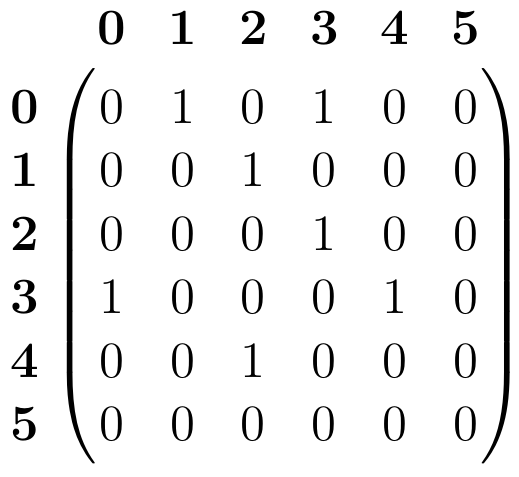
\includegraphics[width=0.48\textwidth]{matrice-di-adiacenza-esempio-1.png}}
    \hfill
    \subfloat[\emph{Lista di adiacenza}]{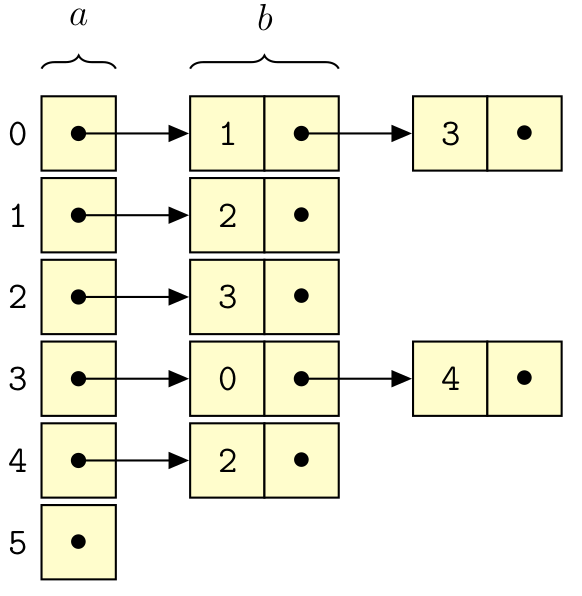
\includegraphics[width=0.48\textwidth]{lista-di-adiacenza-esempio-1.png}}
    \caption{Memorizzazione di un \emph{grafo orientato}}
\end{figure}\noindent
Dall'immagine si può derivare facilmente il \emph{costo di memorizzazione} nei
due casi. Per le \emph{matrici di adiacenza} lo spazio necessario dipende
unicamente dal quadrato del numero di \emph{nodi} e quindi è $O(n^2)$, mentre
per memorizzare una \emph{lista di adiacenza}, lo spazio usato dipende sia dal
numero di \emph{nodi} che di \emph{lati} e quindi è $O(a\cdot n+b\cdot m)=O(n+m)$.

\paragraph{Memorizzazione di un grafo non orientato}
Per i \emph{grafi non orientati} non cambia molto, ma nel caso delle
\emph{matrici di adiacenza} possiamo dimezzare lo spazio grazie alla simmetria
dell'\emph{adiacenza}. Di conseguenza lo spazio necessario diventa $O(\frac{n(n-1)}
{2})$, che però è comunque un $O(n^2)$.

Per le \emph{liste di adiacenza} invece, un \emph{arco} $(u,v)$ deve essere
memorizzato sia tra i \emph{nodi adiacenti} a $u$ che a $v$. Di conseguenza, il
numero di \emph{archi} da memorizzare raddoppia e, conseguentemente, lo spazio
necessario diventa $O(a\cdot n+2b\cdot m)$ che anche sta volte è comunque $O(n+m)$.

\begin{figure}[h!]
    \centering
    \subfloat[\emph{Grafo non orientato}]
    {
        \begin{graph}
            \node[main] (0) {$0$};
            \node[main] (1) [right of=0, xshift=30] {$1$};
            \node[main] (2) [below of=0, yshift=-30] {$3$};
            \node[main] (3) [right of=1, xshift=30] {$2$};
            \node[main] (4) [right of=2, xshift=30] {$4$};
            \node[main] (5) [below of=3, yshift=-30] {$5$};
        
            \draw (0) -- (1);
            \draw (0) -- (2);
            \draw (1) -- (3);
            \draw (2) -- (3);
            \draw (2) -- (4);
            \draw (4) -- (3);
        \end{graph}
    }\\
    \subfloat[\emph{Matrice di adiacenza}]{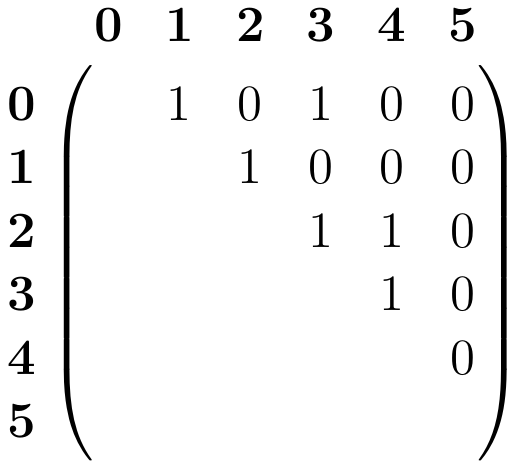
\includegraphics[width=0.48\textwidth]{matrice-di-adiacenza-esempio-1n.png}}
    \hfill
    \subfloat[\emph{Lista di adiacenza}]{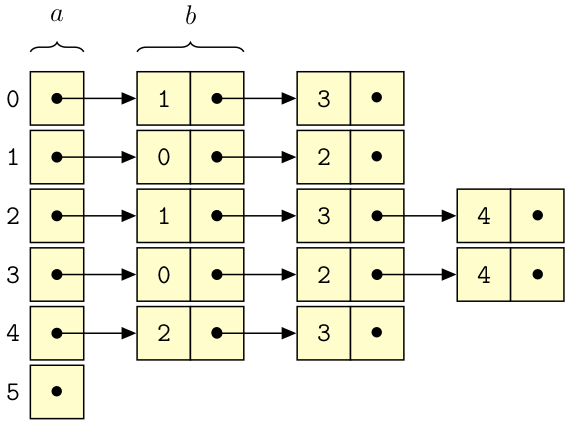
\includegraphics[width=0.48\textwidth]{lista-di-adiacenza-esempio-1n.png}}
    \caption{Memorizzazione di un \emph{grafo non orientato}}
\end{figure}\noindent
Giunti a questo punto possiamo dire che, a parità di metodo di
memorizzazione scelto, lo spazio necessario per memorizzare un \emph{grafo orientato}
non è diverso da quello che servirebbe se il \emph{grafo} fosse \emph{non orientato}.

\paragraph{Memorizzazione di un grafo pesato}
Un caso interessante è quello in cui si debba memorizzare un \emph{grafo pesato},
cioè un \emph{grafo} nel quale ad ogni \emph{arco} è associato un costo (o un
profitto). Matematicamente possiamo pensare il peso di un \emph{arco} come
l'applicazione di una funzione di peso del tipo: $w:\,V\times V\to\mathbb{R}$.
L'unico caso particolare è quello in cui non esista un \emph{arco} tra due
\emph{vertici} e quindi, a seconda del problema che si sta affrontando, si può
decidere di assegnare un peso nullo o infinito.

\noindent
Ciò che cambia nella memorizzazione è che nella \emph{matrice di adiacenza},
invece di indicare un valore binario, si indica il peso dell'\emph{arco}, mentre
nella \emph{lista di adiacenza} si aggiunge il valore del peso all'interno di
ogni \emph{nodo}.

\begin{figure}[h!]
    \centering
    \subfloat[\emph{Grafo pesato non orientato}]
    {
        \begin{graph}
            \node[main] (0) {$0$};
            \node[main] (1) [right of=0, xshift=30] {$1$};
            \node[main] (2) [below of=0, yshift=-30] {$3$};
            \node[main] (3) [right of=1, xshift=30] {$2$};
            \node[main] (4) [right of=2, xshift=30] {$4$};
            \node[main] (5) [below of=3, yshift=-30] {$5$};
        
            \draw (0) -- (1) node [midway, below] {$3$};
            \draw (0) -- (2) node [midway, right] {$1$};
            \draw (1) -- (3) node [midway, below] {$4$};
            \draw (2) -- (3) node [midway, below] {$4$};
            \draw (2) -- (4) node [midway, below] {$8$};
            \draw (4) -- (3) node [midway, below right=-1.5pt] {$7$};
        \end{graph}
    }\\
    \subfloat[\emph{Matrice di adiacenza}]{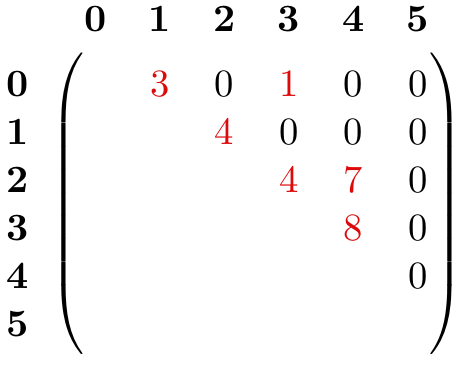
\includegraphics[width=0.48\textwidth]{matrice-di-adiacenza-esempio-1np.png}}
    \hfill
    \subfloat[\emph{Lista di adiacenza}]{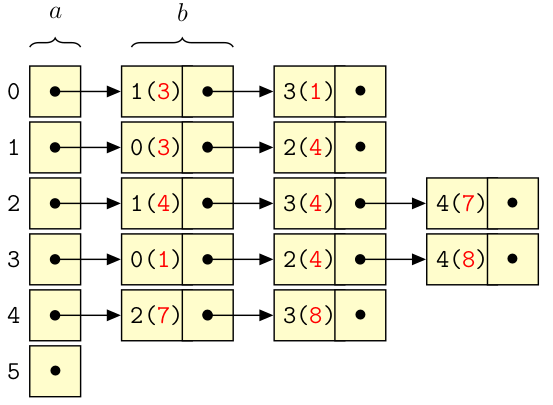
\includegraphics[width=0.48\textwidth]{lista-di-adiacenza-esempio-1np.png}}
    \caption{Memorizzazione di un \emph{grafo pesato non orientato}}
\end{figure}

\paragraph{Dettagli sull'implementazione}
Se non diversamente specificato, di seguito assumeremo che i \emph{grafi} siano
memorizzati come \emph{vettori di adiacenza}, ovvero \emph{liste} implementate
tramite \emph{vettori} (\emph{dinamici} o \emph{statici}). Inoltre, consideriamo
$O(1)$ il costo per l'accesso alle informazioni di un oggetto di classe
\texttt{NODE} e per l'inserimento e la rimozione di \emph{nodi} e \emph{archi}
dai \emph{grafi}. Ipotizzeremo inoltre, che dopo l'inizializzazione i
\emph{grafi} siano \emph{statici} e che quindi non sia più possibile modificarli.

\bigskip\noindent
Fatte queste premesse, possiamo concludere questa sezione discutendo
del \emph{costo} complessivo di alcune operazioni basilari sui \emph{grafi}.

\begin{code}{Iterazione su \emph{nodi} e \emph{archi}}
\begin{minipage}[t]{0.48\textwidth}
\com{Iterazione su tutti i \emph{nodi}}
\rmbreak\ind foreach (u $\in$ G.V()) do\\
    \{ Operazioni sul \emph{nodo} $u$ \}
\end{minipage}
\hfill
\begin{minipage}[t]{0.48\textwidth}
\com{Iterazione su tutti i \emph{nodi} e tutti gli \emph{archi}}
\rmbreak\ind foreach (u $\in$ G.V()) do\\
    \{ Operazioni sul \emph{nodo} $u$ \}\\
    \indf foreach (v $\in$ G.adj(u)) do\\
        \{ Operazioni sull'\emph{arco} $(u,v)$ \}\\
\end{minipage}
\end{code}

\noindent\begin{minipage}[t]{0.48\textwidth}
    \paragraph{Matrici di adiacenza}
    \hbadness=10000
    \begin{itemize}
        \item Lo spazio richiesto per la memorizzazione è $O(n^2)$;
        \item Il tempo richiesto per verificare se un \emph{nodo} $u$ è
        \emph{adiacente} a un altro \emph{nodo} $v$ è $O(1)$;
        \item Il tempo necessario per iterare su tutti gli \emph{archi} è $O(n^2)$
    \end{itemize}
\end{minipage}
\hfill
\begin{minipage}[t]{0.48\textwidth}
    \paragraph{Liste di adiacenza}
    \hbadness=10000
    \begin{itemize}
        \item Lo spazio richiesto per la memorizzazione è $O(n+m)$;
        \item Il tempo richiesto per verificare se un \emph{nodo} $u$ è
        \emph{adiacente} a un altro \emph{nodo} $v$ è $O(n)$;
        \item Il tempo necessario per iterare su tutti gli \emph{archi} è $O(n+m)$
    \end{itemize}
\end{minipage}

\bigskip\noindent
In generale, le \emph{matrici di adiacenza} sono adatte per memorizzare
\emph{grafi densi} e, al contrario, per \emph{grafi sparsi} risulta più
convenienti l'utilizzo delle \emph{liste}.

\section{Visite di un grafo}
\begin{definition}[Visita di un grafo]
    Dati, un grafo $G=(V,E)$ e un vertice $r\in V$ detto radice o sorgente,
    visitare un grafo significa visitare una e una sola volta tutti i nodi del
    grafo che possono essere raggiunti da $r$.
\end{definition}\noindent
Come per gli \emph{alberi}, esistono \emph{visite in profondità} e in
\emph{ampiezza}. Un primo approccio alla \emph{visita} di un \emph{grafo}
potrebbe essere il doppio ciclo visto in precedenza:
\begin{minicode}{Visita scriteriata di un grafo}
\com{Iterazione su tutti i \emph{nodi} e tutti gli \emph{archi}}
\rmbreak\ind foreach (u $\in$ G.V()) do\\
    \{ Operazioni sul \emph{nodo} $u$ \}\\
    \indf foreach (v $\in$ G.adj(u)) do\\
        \{ Operazioni sull'\emph{arco} $(u,v)$ \}
\end{minicode}\noindent
Questo approccio tuttavia non va bene in quanto non viene tenuto conto della struttura
del \emph{grafo} e, cosa più importante, non segue alcun criterio nell'ordine
di visita dei \emph{nodi} e degli \emph{archi}. A dirla tutta, questo approccio
viola la definizione stessa di \emph{visita} in quanto non offre alcuna garanzia
sul fatto che \emph{nodi} e \emph{archi} verranno visitati una sola volta.

\subsection{Visita in ampiezza}
Nella \emph{visita in ampiezza} andiamo a visitare i \emph{nodi} in ordine
crescente di distanza dalla \emph{radice}. Ciò può essere utile per calcolare
il \emph{cammino} più breve da $r$ a tutti gli altri \emph{nodi} e quindi
riuscire a generare un \emph{albero breadth-first}.
\begin{definition}[Albero breadth-first]
    Un albero breadth-first è un albero contenente tutti i nodi raggiungibili da
    $r$ e tale per cui il cammino dalla radice $r$ al nodo $u$ nell'albero
    corrisponde al cammino più breve da $r$ a $u$ nel grafo.
\end{definition}\noindent
Dunque, per l'implementazione della \emph{visita in ampiezza} possiamo partire
da quanto fatto per gli \hyperref[code:15]{\emph{alberi generici}} ipotizzando
di trattare i \emph{nodi adiacenti} come \emph{figli}. Con le opportune
modifiche si ottiene una funzione di questo tipo:
\begin{minicode}{Implementazione errata visita in ampiezza di un grafo}
\ind bfsTraversal(\bc{GRAPH} G, \bc{NODE} r)\\
    \bc{QUEUE} q = Queue()\\
    q.enqueue(r)\\
    \indf while (not q.isEmpty()) do\\
        \bc{NODE} u = q.dequeue()\\
        \{ Visita il \emph{nodo} $u$ \}\\
        \indff foreach (v $\in$ G.adj(u)) do\\
            q.enqueue(v)\hfill\com{Accoda tutti i \emph{nodi adiacenti} a $u$}
\end{minicode}\noindent
Questa implementazione, come la precedente, è errata e il motivo è che non solo
lo stesso \emph{nodo} può essere visitato più volte, ma la funzione non termina
mai l'esecuzione. Infatti, se $u$ e $v$ sono \emph{adiacenti}, quando viene
visitato $u$ viene messo in coda $v$ e quando viene visitato $v$ viene messo in
coda $u$. È quindi necessario utilizzare un sistema che permetta di tenere
traccia dei
\emph{nodi} già visitati.
\begin{minicode}{Implementazione generica visita in ampiezza di un grafo}
\ind graphTraversal(\bc{GRAPH} G, \bc{NODE} r)\\
    \bc{SET} s = Set()\hfill\com{\emph{Insieme} generico}
    s.insert(r)\hfill\com{Da specificare}
    \{ Marca il \emph{nodo} $r$ \}\\
    \indf while (s.size() > 0) do\\
        \bc{NODE} u = s.remove()\hfill\com{Da Specificare}
        \indff foreach (v $\in$ G.adj(u)) do\\
            \{ Visita l'\emph{arco} $(u,v)$ \}\\
            \indfff if (v non è stato ancora marcato) then\\
                \{ Marca il \emph{nodo} $v$ \}\\
                s.insert(v)\hfill\com{Da specificare}
\end{minicode}
\begin{code}{Implementazione visita in ampiezza di un grafo}
\noindent\rmbreak\ind bfs(\bc{GRAPH} G, \bc{NODE} r)\\
    \bc{QUEUE} q = Queue()\\
    q.enqueue(r)\\
    \bc{boolean}[] visited = new \bc{boolean}[G.size()]\hfill\com{\emph{Vettore marcatore}}
    foreach (u $\in$ G.V() - \{r\}) do\hfill\com{Estrae tutti i \emph{nodi} tranne $r$}
        \indf visited[u] = false\\
    \ind visited[r] = true\hfill\com{Marca $r$}
    \ind while (not q.isEmpty()) do\\
        \indf\bc{NODE} u = q.dequeue()\\
        \{ Visita il \emph{nodo} $u$ \}\\
        \indf foreach (v $\in$ G.adj(u)) do\\
            \indff\{ Visita l'\emph{arco} $(u,v)$ \}\\
            if (not visited[v]) then\hfill\com{Controlla se il \emph{nodo} è già stato visitato}
                \indfff visited[v] = true\hfill\com{Marca $v$}
                q.enqueue(v)
\end{code}

\subsection{Visita in profondità}
La \emph{visita in profondità} viene usata per visitare tutti i \emph{nodi} e
non solo quelli raggiungibili da una singola sorgente come avviene con la
\emph{visita in ampiezza}. Proprio per questo, la ricerca restituisce una
\emph{foresta} di \emph{alberi depth-first} e non un solo \emph{albero}.

La funzione \texttt{dfs} per la \emph{visita in profondità} può essere realizzata
in modo ricorsivo o iterativo. In entrambi i casi si fa uso di una \emph{pila},
ma nel caso della ricorsione la \emph{pila} ha una dimensione massima definita
dal sistema operativo, quindi per grafi di grandi dimensioni è bene considerare
attentamente il tipo di implementazione più opportuno.

\begin{minicode}{Implementazione ricorsiva visita in profondità di un grafo}
\ind dfs(\bc{GRAPH} G, \bc{NODE} u, \bc{boolean}[] visited)\\
    visited[u] = true\\
    \{ Visita il \emph{nodo} $u$ \}\hfill\com{Pre-order}
    \indf foreach (v $\in$ G.adj(u)) do\\
        \indff if (not visited[v]) then\\
            \{ Visita l'\emph{arco} $(u,v)$ \}\\
            dfs(G, v, visited)\\

    \indf\{ Visita il \emph{nodo} $u$ \}\hfill\com{Post-order}
\end{minicode}
\begin{minicode}{Implementazione iterativa visita in profondità di un grafo}
\ind dfs(\bc{GRAPH} G, \bc{NODE} u)\\
    \bc{STACK} s = Stack()\\
    s.push(r)\\
    \bc{boolean}[] visited = new \bc{boolean}[G.size()]\\
    \indf foreach (u $\in$ G.V()) do\\
        visited[u] = false\\
    \indf while (not s.isEmpty()) do\\
        \bc{NODE} u = s.pop()\\
        \indff if (not visited[u]) then\\
            \{ Visita il \emph{nodo} $u$ \}\hfill\com{Pre-order}
            visited[u] = true\\
            \indfff foreach (v $\in$ G.adj(u)) do\\
                \{ Visita l'\emph{arco} $(u,v)$ \}\\
                s.push(v)
\end{minicode}\noindent
È bene esplicitare alcuni particolari dell'implementazione iterativa. In
particolare, un \emph{nodo} può essere inserito più volte nella \emph{pila},
in quanto il controllo sul marcatore viene effettuato al momento dell'estrazione
e non dell'inserimento.

La \emph{visita} in \emph{post-order} prevede che alla scoperta di un \emph{nodo}, questo venga inserito nella
\emph{pila} impostando un tag \texttt{discovery}. Alla successiva estrazione di
quel \emph{nodo}, il tag \texttt{discovery} viene cambiato in \texttt{finish} e
il \emph{nodo} viene inserito nuovamente nella \emph{pila}. Alla terza
estrazione viene effettuata la \emph{visita}. L'utilizzo dei tag \texttt{discovery}
e \texttt{finish} garantisce che un \emph{nodo} con tag \texttt{finish} venga
estratto soltanto dopo che tutti i suoi vicini sono già stati inseriti.

\subsection{Complessità delle visite}
Tutte e tre le implementazioni viste per i due tipi di \emph{visite} hanno
\emph{complessità} $O(n+m)$. Nello specifico, l'implementazione iterativa della
\emph{dfs} costa $O(n+m)$ perché effettua $O(m)$ \emph{visite} degli \emph{archi},
$O(m)$ inserimenti ed estrazioni e $O(n)$ \emph{visite} dei \emph{nodi}.

\section{Problemi sui grafi risolubili con visite in ampiezza}
Le \emph{visite in ampiezza} e in \emph{profondità} sono solitamente
sfruttate all'interno di altri algoritmi per risolvere problemi più complessi.

L'utilizzo più importante delle \emph{visite in ampiezza} è nella ricerca del
\emph{cammino più breve} tra due \emph{nodi}. Tuttavia, prima di arrivare a
discutere quel problema, facciamo una piccola digressione e andiamo a vedere
come calcolare la distanza tra un \emph{nodo} e tutti gli altri.

\subsection{Calcolo della distanza tra nodi}
Per distanza tra \emph{nodi} si intende il numero di \emph{archi}
che collegano un \emph{nodo} a tutti gli altri. Il \emph{nodo} di partenza
ha distanza $0$ da se stesso, i suoi vicini, ovvero i \emph{nodi} ad esso
\emph{adiacenti}, hanno distanza $1$ e così via. In generale, se un \emph{nodo}
$u$ è \emph{adiacente} ad un \emph{nodo} che è a distanza $k$ e, contemporaneamente,
non è \emph{adiacente} a nessun \emph{nodo} che ha distanza inferiore a $k$ dal
\emph{nodo} di partenza, allora $u$ è a distanza $k+1$.

\begin{note}
    Il concetto di distanze appena espresso deriva dai cosiddetti \emph{Numeri di
    Erdös}. Erdös fu un matematico estremamente prolifico che scrisse più
    di 1500 articoli con più di 500 coautori. I \emph{numeri di Erdös} descrivono
    la distanza di una persona da Erdös. Quindi, Erdös ha valore $erdos=0$, i
    suoi coautori hanno $erdos=1$ e, in generale, una persona coautore di qualcuno
    con $erdos=k$ e che non è coautore con nessuno che abbia $erdos<k$, ha $erdos=k+1$.
\end{note}\noindent
Quindi, l'algoritmo per il calcolo della distanza di un \emph{nodo} dagli altri,
non fa altro che calcolare il \emph{numero di Erdös} di ogni \emph{nodo}, e lo fa,
sfruttando il meccanismo delle \emph{visite in ampiezza}.

\begin{minicode}{Implementazione distance per il calcolo dei numeri di Erdös}
\ind distance(\bc{GRAPH} G, \bc{NODE} r, \bc{int}[] distances)\\
    \bc{QUEUE} q = Queue()\\
    q.enqueue(r)\\
    \indf foreach (u $\in$ G.V() - \{r\}) do\\
        distances[u] = $\infty$\hfill\com{Tutti i \emph{nodi} non visitati sono a $\infty$}
    \indf distances[r] = 0\\
    \indf while (not q.isEmpty()) do\\
        \bc{NODE} u = q.dequeue()\\
        \indff foreach (v $\in$ G.adj(u)) do\\
            \indfff if (distances[v] == $\infty$) then\hfill\com{Un \emph{nodo} mai visitato ha $erdos=\infty$}
                distances[v] = distance[u] + 1\hfill\com{Se $u$ ha $erdos=k$, $v$ ha $k+1$}
                q.enqueue(v)
\end{minicode}

\subsection{Ricerca del cammino più breve fra due nodi}
Partendo dalla funzione per il calcolo dei \emph{numeri di Erdös} è possibile
implementare una funzione che, dato un \emph{nodo} $r$, costruisca l'\emph{albero
di copertura} con \emph{radice} $r$. Quell'\emph{albero} è realizzato tramite un
\emph{vettore dei padri} e può essere utilizzato per determinare, non solo la
distanza di $r$ da uno dei \emph{nodi}, ma anche il \emph{cammino semplice} più
breve.

\begin{minicode}{Implementazione distance per la ricerca dei cammini brevi}
    \ind distance(\bc{GRAPH} G, \bc{NODE} r, \bc{int}[] distances, \bc{NODE}[] parents)\\
    \bc{QUEUE} q = Queue()\\
    q.enqueue(r)\\
    \indf foreach (u $\in$ G.V() - \{r\}) do\\
        distances[u] = $\infty$\hfill\com{Tutti i \emph{nodi} non visitati sono a $\infty$}
        parents[u] = nil\hfill\com{Tutti i \emph{nodi} non visitati non avranno un \emph{padre}}
    \indf distances[r] = 0\\
    \indf parents[r] = nil\hfill\com{$r$ è la \emph{radice} dell'\emph{albero di copertura}}
\end{minicode}
\begin{codecont}
\begin{minipage}[t]{\textwidth}
    \indf while (not q.isEmpty()) do\\
    \bc{NODE} u = q.dequeue()\\
    \indff foreach (v $\in$ G.adj(u)) do\\
        \indfff if (distances[v] == $\infty$) then\hfill\com{Un \emph{nodo} mai visitato ha $erdos=\infty$}
            distances[v] = distance[u] + 1\hfill\com{Se $u$ ha $erdos=k$, $v$ ha $k+1$}
            parents[v] = u\hfill\com{Popola il vettore dei padri}
            q.enqueue(v)\\
\end{minipage}
\end{codecont}
Il \emph{cammino semplice} tra due \emph{nodi} può poi essere stampato con la
seguente funzione.
\begin{minicode}{Implementazione printPath per la stampa del cammino tra due nodi}
\ind printPath(\bc{NODE} r, \bc{NODE} s, \bc{NODE}[] parents)\\
    \indf if (r == s) then\hfill\com{\emph{Cammino} tra un \emph{nodo} e se stesso}
        print s\\
    \indf else if (parents[s] == nil) then\hfill\com{Se il \emph{padre} è \texttt{nil}, non esiste un \emph{cammino}}
        print "error"\\
    \indf else\\
        printPath(r, parents[s], parents)\\
        print s
\end{minicode}

\paragraph{Complessità}
Entrambe le funzioni hanno \emph{complessità lineare} $O(n+m)$ perché si basano
sull'algoritmo per la \emph{visita in ampiezza}.

\section{Problemi sui grafi risolubili con visite in profondità}
\subsection{Ricerca delle componenti connesse}
\begin{definition}[Raggiungibilità]
    Un nodo $v$ è raggiungibile da un nodo $u$ se esiste almeno un cammino da
    $u$ a $v$.
\end{definition}
\begin{note}
    Nei \emph{grafi non orientati} il concetto di \emph{raggiungibilità} è
    simmetrico.
\end{note}
\begin{definition}[Grafo connesso]
    Un grafo non orientato $G=(V,E)$ è connesso se e solo se ogni suo nodo
    è raggiungibile da ogni altro nodo.
\end{definition}
\begin{definition}[Sottografo]
    $G'=(V',E')$ è un sottografo di $G=(V,E)$, ovvero $G'\subseteq G$ se e solo
    se $V'\subseteq V$ e $E'\subseteq E$.
\end{definition}
\begin{definition}[Grafo massimale]
    $G'$ è massimale se e solo se non esiste un altro sottografo $G''$ di $G$
    che sia connesso e più grande di $G'$, ovvero se non esiste un grafo $G''$
    che soddisfi la seguente relazione:
    \[G'\subseteq G''\subseteq G\]
\end{definition}
\begin{definition}[Componente connessa]
    Un grafo $G'=(V', E')$ è una componente connessa di $G=(V,E)$ se e solo se
    è un sottografo connesso e massimale di $G$.
\end{definition}\noindent
Fatte salve queste definizioni, possiamo dire che una \emph{visita in profondità}
può sia permetterci di capire se un grafo è \emph{connesso} o meno, che di
conoscere le sue \emph{componenti connesse}. Per fare ciò, è sufficiente usare
un \emph{vettore} contenente gli identificatori delle \emph{componenti connesse}.
In particolare, il valore in posizione $u$ del \emph{vettore} è l'identificatore
della \emph{componente connessa} alla quale appartiene il \emph{nodo} $u$.

\begin{minicode}{Implementazione cc per la ricerca delle componenti connesse}
\ind\bc{int}[] cc(\bc{GRAPH} G)\\
    \bc{int}[] id = new \bc{int}[G.size()]\hfill\com{\emph{Vettore} degli identificatori}
    \indf foreach (u $\in$ G.V()) do\\
        id[u] = 0\\
    \indf\bc{int} counter = 0\hfill\com{Contatore \emph{Componenti Connesse}}
    \indf foreach (u $\in$ G.V()) do\\
        \indff if (id[u] == 0) then\\
            counter = counter + 1\\
            ccdfs(G, counter, u, id)\\
    \indf return id

\nl\com{Funzione ausiliaria che marca tutti i \emph{nodi} tra loro \emph{raggiungibili}}
\rmbreak\ind ccdfs(\bc{GRAPH} G, \bc{int} counter, \bc{NODE} u, \bc{int}[] id)\\
    id[u] = counter\\
    \indf foreach (v $\in$ G.adj(u)) do\\
        \indff if (id[v] == 0) then\\
            ccdfs(G, counter, v, id)
\end{minicode}
\newpage
\begin{figure}[ht]
    \centering
    \begin{graph}
        \node[main, label=$1$] (0) {$a$};
        \node[main, label=$1$] (1) [right of=0, xshift=30] {$b$};
        \node[main, label=$1$] (2) [right of=1, xshift=30] {$c$};
        \node[main, label=below:$1$] (3) [below of=1, yshift=-30] {$d$};
    
        \path[->] (0) edge[bend left=15] (1)
                  (1) edge[bend left=15] (2)
                  (2) edge[bend left=15] (3);
    
        \path[<-, dashed] (0) edge[bend right=15] (1)
                  (1) edge[bend right=15] (2)
                  (2) edge[bend right=15] (3)
                  (1) edge[bend right=15] (3)
                  (3) edge[bend right=15] (1)
                  (0) edge[bend right=15] (3)
                  (3) edge[bend right=15] (0);
    
        \node[main, label=$2$] (4) [right of=2, xshift=30] {$e$};
        \node[main, label=$2$] (5) [right of=4, xshift=30] {$f$};
        \node[main, label=$2$] (6) [below right of=5, xshift=30] {$i$};
        \node[main, label=below:$2$] (7) [below of=4, yshift=-30] {$g$};
        \node[main, label=below:$2$] (8) [right of=7, xshift=30] {$h$};
    
        \path[->] (4) edge[bend left=15] (5)
                  (5) edge[bend left=15] (8)
                  (8) edge[bend left=15] (6)
                  (8) edge[bend left=15] (7);
    
        \path[<-, dashed] (4) edge[bend right=15] (5)
                  (5) edge[bend right=15] (8)
                  (8) edge[bend right=15] (6)
                  (8) edge[bend right=15] (7)
                  (4) edge[bend right=15] (7)
                  (7) edge[bend right=15] (4)
                  (5) edge[bend right=15] (6)
                  (6) edge[bend right=15] (5);
    
        \node[main, label=$3$] (9) [below right of=3, xshift=30, yshift=-30] {$j$};
        \node[main, label=$3$] (10) [right of=9, xshift=30] {$k$};
    
        \draw[->] (9) edge[bend left=15] (10);
        \draw[<-, dashed] (9) edge[bend right=15] (10);
    \end{graph}
    \caption{\emph{Grafo} con tre \emph{componenti connesse}}
\end{figure}
\begin{note}
    Nella figura di cui sopra è rappresentato un \emph{grafo orientato}, ma
    poiché per ogni coppia di \emph{nodi} esiste un \emph{arco} in entrambe le
    direzioni, il \emph{grafo} può anche essere visto come \emph{non
    orientato}.
\end{note}

\subsection{Verifica di esistenza di cicli nei grafi non orientati}
\begin{definition}[Ciclo in un grafo non orientato]
    In grafo non orientato $G=(V,E)$, un ciclo $C$ di lunghezza $k>2$ è una
    sequenza di nodi $u_0,\,u_1\,\dots,\,u_k$ tale che $(u_i,\,u_{i+1})\in E$
    $\forall\,0\leq i\leq k-1$ e $u_0=u_k$.
\end{definition}
\begin{note}
    Il vincolo $k>2$ serve per escludere i \emph{cicli} banali composti da
    coppie di \emph{archi} $(u,v)$ e $(v,u)$ che sono onnipresenti nei
    \emph{grafi non orientati}.
\end{note}

\begin{definition}[Grafo aciclico]
    Un grafo non orientato che non contiene cicli è detto aciclico.
\end{definition}
\begin{definition}[Grafo ciclico]
    Un grafo che contiene almeno un ciclo è detto essere ciclico.
\end{definition}\noindent
Riuscire a capire se un \emph{grafo non orientato} contiene cicli, non è
difficile. È sufficiente modificare l'algoritmo per la \emph{visita in
profondità} aggiungendo un parametro che ad ogni invocazione contenga un
riferimento all'ultimo \emph{nodo} visitato. Quindi, si esegue la normale
\emph{visita in profondità}, evitando però di visitare il \emph{nodo} indicato
dal parametro, e, se si arriva a un altro \emph{nodo} già visitato, allora si è
in presenza di un \emph{ciclo}.

\begin{code}{Implementazione hasCycle per la verifica di esistenza di
    cicli in grafi non orientati}
\noindent\rmbreak\ind\bc{boolean} hasCycle(\bc{GRAPH} G)\\
    \bc{boolean}[] visited = new \bc{boolean}[G.size()]\\
    foreach (u $\in$ G.V()) do\\
        \indf visited[u] = false\\
    \ind foreach (u $\in$ G.V()) do\\
        \indf if (not visited[u]) then\\
            \indff if (hasCycleRec(G, u, nil, visited)) then\\
                \indfff return true\\
    \ind return false\\

\noindent\com{Funzione ausiliaria}
\rmbreak\ind\bc{boolean} hasCycleRec(\bc{GRAPH} G, \bc{NODE} u, \bc{NODE} p, \bc{boolean}[] visited)\\
    visited[u] = true\\
    foreach (v $\in$ G.adj(u) - \{p\}) do\hfill\com{Visita tutti i \emph{nodi} adiacenti tranne $p$}
        \indf if (visited[v]) then\\
            \indff return true\\
        \indf else if (hasCycleRec(G, v, u, visited)) then\\
            \indff return true\\
    \ind return false
\end{code}

\subsection{Verifica di esistenza di cicli nei grafi orientati}
\begin{definition}[Ciclo in un grafo orientato]
    In un grafo orientato $G=(V,E)$, un ciclo $C$ di lunghezza $k\geq 2$ è
    una sequenza di nodi $u_0,\,u_1,\,\dots,\,u_k$ tale che $(u_i,\,u_{i+1})\in E$
    $\forall\,0\leq i\leq k-1$ e $u_0=u_k$.
\end{definition}
\begin{note}
    Nei \emph{grafi orientati} i \emph{cicli} banali formati da coppie di
    \emph{archi} $(u,v)$ e $(v,u)$ sono accettati.
\end{note}
\begin{note}
    I \emph{cicli} in cui tutti i \emph{nodi} ad eccezione del primo e l'ultimo
    sono distinti sono detti \emph{cicli semplici}.
\end{note}
\begin{definition}[Grafi orientati aciclici - DAG]
    Un grafo orientato che non contiene cicli è detto essere un DAG (Directed
    Acyclic Graph).
\end{definition}

\begin{figure}[h!]
    \centering
    \subfloat[\emph{Grafo DAG}]
    {
        \resizebox*{0.42\textwidth}{!}{
        \begin{graph}
            \node[main] (0) {$a$};
            \node[main] (1) [above right of=0, xshift=20, yshift=10] {$b$};
            \node[main] (2) [below right of=0, xshift=20, yshift=-10] {$d$};
            \node[main] (3) [right of=1, xshift=20] {$c$};
            \node[main] (4) [right of=2, xshift=20] {$e$};
            \node[main] (5) [below right of=3, xshift=20, yshift=-10] {$f$};
          
            \draw[->] (0) -- (1);
            \draw[->] (0) -- (2);
            \draw[->] (1) -- (3);
            \draw[->] (2) -- (3);
            \draw[->] (2) -- (4);
            \draw[->] (3) -- (4);
            \draw[->] (3) -- (5);
            \draw[->] (4) -- (5);
        \end{graph}}
    }
    \hspace{1.5cm}
    \subfloat[\emph{Grafo ciclico}]
    {
        \resizebox*{0.42\textwidth}{!}{
        \begin{graph}
            \node[main] (0) {$a$};
            \node[main] (1) [above right of=0, xshift=20, yshift=10] {$b$};
            \node[main] (2) [below right of=0, xshift=20, yshift=-10] {$d$};
            \node[main] (3) [right of=1, xshift=20] {$c$};
            \node[main] (4) [right of=2, xshift=20] {$e$};
            \node[main] (5) [below right of=3, xshift=20, yshift=-10] {$f$};
          
            \draw[->] (0) -- (1);
            \draw[->] (0) -- (2);
            \draw[->] (1) -- (3);
            \draw[->, line width=1.3pt] (2) -- (3);
            \draw[->, line width=1.3pt] (4) -- (2);
            \draw[->, line width=1.3pt] (3) -- (4);
            \draw[->] (3) -- (5);
            \draw[->] (4) -- (5);
        \end{graph}}
    }
    \caption{\emph{Grafi DAG} VS \emph{grafi ciclici}}
\end{figure}\noindent
Verificare l'esistenza di \emph{cicli} all'interno di \emph{grafi orientati}
non è semplice come nei \emph{grafi non orientati}, infatti non è possibile
usare l'algoritmo visto in precedenza, ma ne serve uno ad-hoc.

\begin{definition}[Archi degli alberi di copertura]
    Ogni volta che si esamina un arco da un nodo marcato a uno non marcato, tale
    arco viene detto arco dell'albero.
\end{definition}\noindent
Quando si effettua una \emph{visita}, l'\emph{albero di copertura} risultante
non contiene tutti gli \emph{archi} del \emph{grafo}. Gli \emph{archi} $(u,v)$ non
compresi nell'\emph{albero di copertura} $T$ possono essere classificati in tre modi:
\begin{itemize}
    \item Se $u$ è un antenato di $v$ in $T$, $(u,v)$ è detto \emph{arco in avanti};
    \item Se $u$ è un discendente di $v$ in $T$, $(u,v)$ è detto \emph{arco all'indietro};
    \item Se $(u,v)$ non è né un \emph{arco in avanti}, né un \emph{arco
    all'indietro}, è un \emph{arco di attraversamento};
\end{itemize}

\vspace*{-0.5cm}
\begin{figure}[ht]
    \centering
    \subfloat[\emph{Grafo orientato}]
    {
        \begin{graph}
            \node[main] (0) [yshift=-20] {$a$};
            \node[main] (1) [right of=0, xshift=30] {$b$};
            \node[main] (2) [below of=0, yshift=-30] {$c$};
            \node[main] (3) [right of=2, xshift=30] {$d$};
            
            \path[->] (0) edge (1)
                        (0) edge (3)
                        (1) edge (2)
                        (3) edge (1)
                        (3) edge (2)
                        (0) edge[bend left=15] (2)
                        (2) edge[bend left=15] (0);

            \node[] (4) at (3) [yshift=-10] {};
        \end{graph}
    }
    \hspace{2.5cm}
    \subfloat[\emph{Albero di copertura con radice $a$}]
    {
        \begin{graph}
            \node[main] (0) {$a$};
            \node[main] (1) [below left of=0, yshift=-15, xshift=5] {$b$};
            \node[main] (2) [below right of=0, yshift=-15, xshift=-5] {$c$};
            \node[main] (3) [below right of=1, yshift=-15, xshift=-15] {$d$};
            
            \path[->, color=red]    (0) edge (1)
                                    (0) edge (2)
                                    (1) edge (3);
            \path[->, dashed, color=blue]   (2) edge (1)
                                            (2) edge (3);
            \draw[->, dashed, color=Dandelion] (3) -- (0);
            \draw[->, dashed, color=Purple] (0) edge[bend right=90] (3);

            \node[] (4) [right of=2, xshift=-25] {};
            \node[] (5) [left of=1, xshift=10] {};
        \end{graph}
    }
    \caption{\emph{Classificazione degli archi}}
\end{figure}\noindent
Nella figura si vede l'\emph{albero di copertura} ottenuto dopo aver effettuato una
\emph{visita in profondità} partendo dal \emph{nodo} $a$. Gli \emph{archi} rossi
sono gli \emph{archi dell'albero di copertura}, mentre gli \emph{archi} $(a,d)$
e $(d,a)$ sono, rispettivamente, un \emph{arco in avanti} e un \emph{arco
all'indietro}. Infine, gli \emph{archi} uscenti da $c$ sono \emph{archi di
attraversamento}.

\begin{code}{Implementazione dfs\_schema per la classificazione degli archi}
\noindent\rmbreak\ind dfs\_schema(\bc{GRAPG} G, \bc{NODE} u, \bc{int} \&time, \bc{int}[] dt, \bc{int}[] ft)\\
    time = time + 1\hfill\com{Aggiorna il contatore del tempo}
    dt[u] = time\hfill\com{Imposta il tempo di scoperta del \emph{nodo} $u$}
    foreach (v $\in$ G.adj(u)) do\\
        \indf if (dt[v] == 0) then\hfill\com{\emph{Arco dell'albero}}
            \indff\{ Visita l'\emph{arco} $(u,v)$ \}\\
            dfs\_schema(G, v, time, dt, ft)\\
        \indf else if (dt[u] > dt[v] and ft[v] == 0) then\hfill\com{\emph{Arco all'indietro}}
            \indff\{ Visita l'\emph{arco} $(u,v)$ \}\\
        \indf else if (dt[u] < dt[v] and ft[v] $\neq$ 0) then\hfill\com{\emph{Arco in avanti}}
            \indff\{ Visita l'\emph{arco} $(u,v)$ \}\\
        \indf else\hfill\com{\emph{Arco di attraversamento}}
            \indff \{ Visita l'\emph{arco} $(u,v)$ \}\\
    \ind time = time + 1\hfill\com{Aggiorna il contatore del tempo}
    \ind ft[u] = time\hfill\com{Imposta il tempo di fine visita del \emph{nodo} $u$}
\end{code}\noindent
In questa funzione, il \emph{tempo di scoperta} viene impostato quando per la prima
volta si visita un \emph{nodo}, mentre il \emph{tempo di fine visita} quando sono
già stati visitati tutti i \emph{nodi adiacenti}.

\begin{definition}[Teorema di caratterizzazione delle coppie di nodi]
    Data una visita in profondità di un grafo $G=(V,E)$, per ogni coppia di nodi
    $u,\,v\in V$, vale una delle seguenti condizioni:
    \begin{itemize}
        \item Gli intervalli $[dt[u],\,ft[u]]$ e $[dt[v],\,ft[v]]$ non si
        intersecano, né sovrappongono in alcun modo dunque, $u$ e $v,$ nella
        foresta depth-first, non sono discendenti l'uno dell'altro;
        \item L'intervallo $[dt[u],\,ft[u]]$ è contenuto in $[dt[v],\,ft[v]]$
        dunque, in uno degli alberi depth-first, $u$ è un discendente di $v$;
        \item L'intervallo $[dt[u],\,ft[u]]$ contiene $[dt[v],\,ft[v]]$
        dunque, in uno degli alberi depth-first, $u$ è un antenato di $v$;
    \end{itemize}
\end{definition}\noindent
Grazie a questa definizione possiamo dire che, dati due \emph{nodi} $u$ e $v$, se
vale la seguente:
\[[dt[u],\,ft[u]]\subset[dt[v],\,ft[v]]\]
valgono le seguenti affermazioni:
\begin{itemize}
    \item Il \emph{nodo} $v$ è un \emph{antenato} di $u$;
    \item Il \emph{nodo} $u$ è un \emph{discendente} di $v$;
    \item L'\emph{arco} $(v,u)$, se non è un \emph{arco dell'albero}, è un
    \emph{arco in avanti};
    \item L'\emph{arco} $(u,v)$, se non è un \emph{arco dell'albero}, è un
    \emph{arco all'indietro};
\end{itemize}

\begin{figure}[h!]
    \centering
    \begin{graph}
        \node[main, label={$[6,7]$}] (0) {$d$};
        \node[main, label=right:{$[2,5]$}] (1) [below of=0, yshift=-20] {$b$};
        \node[main, label={$[1,8]\ $}] (2) [left of=1, xshift=-20] {$a$};
        \node[main, label=below:{$[3,4]$}] (3) [below of=1, yshift=-20] {$c$};
        \node[main, label=below:{$[9,10]$}] (4) [left of=3, xshift=-20] {$e$};
      
        \path[->, color=red] (2) edge[bend left=15] (0)
                                  (2) edge (1)
                                  (1) edge (3);
        \path[->, dashed, color=blue] (0) edge (1)
                                  (4) edge (3);
        \draw[->, dashed, color=Dandelion] (0) edge[bend left=15] (2);
        \draw[->, dashed, color=Purple] (2) -- (3);
    \end{graph}
    \caption{Classificazione degli \emph{archi} e intervalli di tempo}
\end{figure}\noindent
Nella figura di cui sopra, si è effettuata una \emph{visita in profondità} a
partire dal \emph{nodo} $a$ e si sono visitati, nell'ordine, i \emph{nodi}
$a$, $b$, $c$, $d$. Gli \emph{archi} $(a,b)$, $(b,c)$ e $(a,d)$ sono \emph{archi
dell'albero} poiché quando $b$, $c$ e $d$ sono stati scoperti avevano certamente
$dt=0$.

L'intervallo associato al \emph{nodo} $d$ è contenuto in quello associato
al \emph{nodo} $a$, quindi l'\emph{arco} $(d,a)$, poiché non è un \emph{arco
dell'albero}, è un \emph{arco all'indietro}. In realtà, quando l'algoritmo
arriva a visitare il \emph{nodo} $d$, $ft[a]$ non è ancora stato impostato, ma
dato che la condizione \texttt{dt[u] > dt[v] and ft[v] == 0} con $u=d$ e $v=a$
risulta verificata, l'\emph{arco} ($d,a$) è effettivamente un \emph{arco
all'indietro}.

\noindent
L'\emph{arco} $(a,c)$, invece, è un \emph{arco in avanti} perché verifica la
relazione sugli intervalli, ovvero $[dt[c],\,ft[c]]\subset[dt[a],\,ft[a]]$, ma
anche perché durante l'esecuzione dell'algoritmo la condizione \texttt{dt[u] <
dt[v] and ft[v] $\neq$ 0} con $u=a$ e $v=c$ viene verificata.

Infine, il \emph{nodo} $e$ non appartiene alla \emph{componente connessa} di
$a$, quindi non fa nemmeno parte dello stesso \emph{albero di copertura}.
L'\emph{arco} $(e,c)$ non soddisfa nessuna condizione quindi è un \emph{arco di
attraversamento}.

\bigskip\noindent
Fatta questa digressione, possiamo ritornare al problema originale:
verificare l'esistenza di \emph{cicli} in un \emph{grafo orientato}.
Enunciamo il seguente teorema.
\begin{definition}[Teorema di esistenza dei cicli]
    Un grafo orientato è aciclico se e solo se non esistono archi all'indietro.
\end{definition}
\begin{proof}[Dimostrazione]
    \mbox{}
    \begin{itemize}
        \item $(\Rightarrow)$: si supponga esista un \emph{ciclo}. Sia $(v,u)$ un
        \emph{arco} del \emph{ciclo} e sia $u$ il primo \emph{nodo} ad essere visitato.
        Prima o poi verrà visitato il \emph{cammino} che connette $u$ a $v$ e da $v$
        verrà scoperto l'\emph{arco all'indietro} $(v,u)$;
        \item $(\Leftarrow)$: se esiste un \emph{arco all'indietro} $(u,v)$, dove
        $v$ è un antenato di $u$, allora esistono un \emph{cammino} da $v$ a $u$
        e un \emph{arco} da $u$ a $v$, ovvero un \emph{ciclo};
    \end{itemize}
\end{proof}\noindent
Quindi, per verificare l'esistenza di un \emph{ciclo} è sufficiente cercare un
\emph{arco all'indietro}. Se ne esiste almeno uno, esisterà sicuramente un anche
un \emph{ciclo}.

\begin{minicode}{Implementazione hasCycle per la verifica di esistenza di cicli
    in un grafo orientato}
\ind\bc{boolean} hasCycle(\bc{GRAPH} G, \bc{NODE} u, \bc{int} \&time, \bc{int}[] dt, \bc{int}[] ft)\\
    time = time + 1\\
    dt[u] = time\\
    \indf foreach (v $\in$ G.adj(u)) do\\
        \indff if (dt[v] == 0) then\\
            \indfff if (hasCycle(G, v, time, dt, ft)) then\\
                return true\\
        \indff else if (dt[u] > dt[v] and ft[v] == 0) then\\
            return true\\
    \indf time = time + 1\\
    \indf ft[u] = time\\
    \indf return false
\end{minicode}

\subsection{Realizzare un ordinamento topologico di un grafo orientato}
\begin{definition}[Ordinamento topologico]
    Dato un grafo orientato aciclico (DAG) $G$, un ordinamento topologico di $G$
    è un ordinamento lineare dei suoi nodi tale che se $(u,v)\in E$, allora $u$
    appare prima di $v$ nell'ordinamento.
\end{definition}

\newpage
\begin{note}
    Se il \emph{grafo} è \emph{aciclico} esistono più ordinamenti possibili, ma
    se esiste anche solo un \emph{ciclo} non ne esiste alcuno.
\end{note}

\begin{figure}[ht]
    \centering
    \begin{graph}
        \node[main] (0) {$1$};
        \node[main] (1) [right of=0, xshift=10] {$3$};
        \node[main] (2) [above of=1, yshift=10] {$2$};    
        \node[main] (3) [below of=1, yshift=-10] {$5$};
        \node[main] (4) [right of=1, xshift=10] {$4$};
    
        \path[->] (0) edge (1)
                  (0) edge (2)
                  (0) edge (3)
                  (1) edge (3)
                  (2) edge (4);
    
        \node[main] (5) [above right of=4, yshift=15, xshift=15] {$1$};
        \node[main] (6) [right of=5, xshift=10] {$3$};
        \node[main] (7) [right of=6, xshift=10] {$5$};
        \node[main] (8) [right of=7, xshift=10] {$2$};
        \node[main] (9) [right of=8, xshift=10] {$4$};
    
        \path[->] (5) edge (6)
                  (6) edge (7)
                  (5) edge[bend left=30] (7)
                  (5) edge[bend right=30] (8)
                  (8) edge (9);
    
        \node[main] (10) [below right of=4, yshift=-15, xshift=15] {$1$};
        \node[main] (11) [right of=10, xshift=10] {$2$};
        \node[main] (12) [right of=11, xshift=10] {$3$};
        \node[main] (13) [right of=12, xshift=10] {$4$};
        \node[main] (14) [right of=13, xshift=10] {$5$};
    
        \path[->] (10) edge (11)
                  (10) edge[bend left=30] (12)
                  (10) edge[bend left=45] (14)
                  (11) edge[bend right=45] (13)
                  (12) edge[bend right=45] (14);
    \end{graph}
    \caption{Possibili \emph{ordinamenti topologici} di un \emph{grafo}}
\end{figure}

\vspace{-0.7cm}
\paragraph{Approccio naive}
Un primo approccio a questo problema potrebbe essere quello in cui, scelto un
\emph{nodo} privo di \emph{archi entranti}, lo si aggiunge all'ordinamento e si
rimuovono tutti i suoi \emph{archi}. Quindi, si ripete l'operazione per tutti
gli altri \emph{nodi}.

\begin{figure}[h!]
    \centering
    \subfloat[Output: ]
    {
        \begin{graph}
            \node[main] (0) {$1$};
            \node[main] (1) [right of=0, xshift=10] {$3$};
            \node[main] (2) [above of=1, yshift=10] {$2$};    
            \node[main] (3) [below of=1, yshift=-10] {$5$};
            \node[main] (4) [right of=1, xshift=10] {$4$};

            \path[->] (0) edge (1)
                    (0) edge (2)
                    (0) edge (3)
                    (1) edge (3)
                    (2) edge (4);
        \end{graph}
    }
    \subfloat[Output: 1]
    {
        \begin{graph}
            \node[] (0) {};
            \node[main] (1) [right of=0, xshift=10] {$3$};
            \node[main] (2) [above of=1, yshift=10] {$2$};    
            \node[main] (3) [below of=1, yshift=-10] {$5$};
            \node[main] (4) [right of=1, xshift=10] {$4$};

            \path[->] (1) edge (3)
                    (2) edge (4);
        \end{graph}
    }
    \subfloat[Output: 1 3]
    {
        \begin{graph}
            \node[] (0) {};
            \node[] (1) [right of=0, xshift=10] {};
            \node[main] (2) [above of=1, yshift=10] {$2$};    
            \node[main] (3) [below of=1, yshift=-10] {$5$};
            \node[main] (4) [right of=1, xshift=10] {$4$};
    
            \path[->] (2) edge (4);
        \end{graph}
    }
    \hfill
\end{figure}

\begin{figure}[h!]
    \ContinuedFloat
    \centering
    \subfloat[Output: 1 3 5]
    {
        \begin{graph}
            \node[] (0) {};
            \node[] (1) [right of=0, xshift=10] {};
            \node[main] (2) [above of=1, yshift=10] {$2$};    
            \node[] (3) [below of=1, yshift=-10] {};
            \node[main] (4) [right of=1, xshift=10] {$4$};
    
            \path[->] (2) edge (4);
        \end{graph}
    }
    \subfloat[Output: 1 3 5 2]
    {
        \begin{graph}
            \node[] (0) {};
            \node[] (1) [right of=0, xshift=10] {};
            \node[] (2) [above of=1, yshift=10] {};
            \node[] (3) [below of=1, yshift=-10] {};
            \node[main] (4) [right of=1, xshift=10] {$4$};
        \end{graph}
    }
    \subfloat[Output: 1 3 5 2 4]
    {
        \begin{graph}
            \node[] (0) {};
            \node[] (1) [right of=0, xshift=10] {};
            \node[] (2) [above of=1, yshift=10] {};
            \node[] (3) [below of=1, yshift=-10] {};
            \node[] (4) [right of=1, xshift=10] {};
        \end{graph}
    }
    \caption{Esecuzione dell'algoritmo \q{naive} per l'\emph{ordinamento topologico}}
\end{figure}

\paragraph{Approccio efficiente}
Un approccio migliore prevede di effettuare una \emph{visita in Post-order}
inserendo tutti i \emph{nodi} in una \emph{pila} a mano a mano che li si visita.
L'utilizzo della \emph{visita in Post-order} fa si che un \emph{nodo} venga
inserito solo quando tutti i suoi \emph{discendenti} sono già stati scoperti ed
aggiunti alla \emph{pila}, e, l'utilizzo della \emph{pila} permette di estrarre
i \emph{nodi} in ordine inverso a quello di \emph{inserimento}. Ciò, permette di
ottenere un corretto \emph{ordinamento topologico}.

\begin{minicode}{Implementazione topSort per l'ordinamento topologico di un grafo DAG}
\ind\bc{STACK} topSort(\bc{GRAPH} G)\\
    \bc{STACK} s = Stack()\\
    \bc{boolean}[] visited = new \bc{boolean}[G.size()]\\
    \indf foreach (u $\in$ G.V()) do\\
        visited[u] = false\\
    \indf foreach (u $\in$ G.V()) do\\
        \indff if (not visited[u]) then\\
            ts-dfs(G, u, visited, s)\hfill\com{Effettua la \emph{visita in Post-order}}
    \indf return s\\

\com{Funzione ausiliaria}
\rmbreak\ind ts-dfs(\bc{GRAPH} G, \bc{NODE} u, \bc{boolean}[] visited, \bc{STACK} s)\\
    visited[u] = true\\
    \indf foreach (v $\in$ G.adj(u)) do\\
        \indff if (not visited[v]) then\\
            ts-dfs(G, v, visited, s)\\
    \indf s.push(u)
\end{minicode}

\begin{figure}[ht]
    \centering
    \subfloat[\emph{Ordinamento topologico} partendo da $1$]
    {
        \begin{graph}
            \node[main, label={$[1,10]$}] (0) {$1$};
            \node[main, label={$[2,5]$}] (1) [right of=0, xshift=10] {$3$};
            \node[main, label={$[6,9]$}] (2) [above of=1, yshift=10] {$2$};    
            \node[main, label=below:{$[3,4]$}] (3) [below of=1, yshift=-10] {$5$};
            \node[main, label={$[7,8]$}] (4) [right of=1, xshift=10] {$4$};
        
            \path[->, color=red] (0) edge (1)
                      (0) edge (2)
                      (1) edge (3)
                      (2) edge (4);
            \draw[->, dashed, color=Purple] (0) -- (3);
        
            \node[] (5) [right of=4, xshift=-17] {};
            \node[] (6) [left of=0, xshift=17] {};

            \node[] (7) [below of=3] {\texttt{Stack = \{1, 2, 4, 3, 5\}}};
        \end{graph}
    }
    \hfill
    \subfloat[\emph{Ordinamento topologico} partendo da $5$]
    {
        \begin{graph}
            \node[main, label={$[9,10]$}] (0) {$1$};
            \node[main, label={$[3,4]$}] (1) [right of=0, xshift=10] {$3$};
            \node[main, label={$[7,8]$}] (2) [above of=1, yshift=10] {$2$};    
            \node[main, label=below:{$[1,2]$}] (3) [below of=1, yshift=-10] {$5$};
            \node[main, label={$[5,6]$}] (4) [right of=1, xshift=10] {$4$};
        
            \path[->] (0) edge (1)
                      (0) edge (2)
                      (1) edge (3)
                      (2) edge (4)
                      (0) edge (3);

            \node[] (5) [right of=4, xshift=-17] {};
            \node[] (6) [left of=0, xshift=17] {};
        
            \node[] (7) [below of=3] {\texttt{Stack = \{1, 2, 4, 3, 5\}}};
        \end{graph}
    }
    \caption{Esempi di \emph{ordinamenti topologici}}
\end{figure}

\newpage
\subsection{Ricerca delle componenti fortemente connesse}
\begin{definition}[Grafo fortemente connesso]
    Un grafo orientato $G=(V,E)$ è fortemente connesso se e solo se ogni suo
    nodo è raggiungibile da ogni altro nodo.
\end{definition}
\begin{definition}[Componente fortemente connessa]
    Un grafo $G'=(V',E')$ è una componente fortemente connessa di $G=(V,E)$ se
    e solo se $G'$ è un sottografo fortemente connesso e massimale di $G$.
\end{definition}

\begin{figure}[h!]
    \centering
    \subfloat[\emph{Grafo orientato}]
    {
        \begin{graph}
            \node[main] (0) {$a$};
            \node[main] (1) [above right of=0, xshift=20, yshift=10] {$b$};
            \node[main] (2) [below right of=0, xshift=20, yshift=-10] {$d$};
            \node[main] (3) [right of=1, xshift=20] {$c$};
            \node[main] (4) [right of=2, xshift=20] {$e$};
            \node[main] (5) [below right of=3, xshift=20, yshift=-10] {$f$};
          
            \draw[->] (0) -- (1);
            \draw[->] (0) -- (2);
            \draw[->] (1) -- (3);
            \draw[->] (2) -- (3);
            \draw[->] (4) -- (2);
            \draw[->] (3) -- (4);
            \draw[->] (4) -- (5);
            \draw[->] (5) -- (3);

            \node[] (6) [below of=2, yshift=23] {};
        \end{graph}
    }
    \hfill
    \subfloat[\emph{Componenti fortemente connesse}]
    {
        \begin{graph}
            \node[main] (0) {$a$};
            \node[main] (1) [above right of=0, xshift=20, yshift=10] {$b$};
            \node[main] (2) [below right of=0, xshift=20, yshift=-10] {$d$};
            \node[main] (3) [right of=1, xshift=20] {$c$};
            \node[main] (4) [right of=2, xshift=20] {$e$};
            \node[main] (5) [below right of=3, xshift=20, yshift=-10] {$f$};
          
            \draw[color=red, dashed, line width=1.3pt] (0) circle (0.6);
            \draw[color=red, dashed, line width=1.3pt] (1) circle (0.6);
            \draw[color=red, dashed, line width=1.3pt, rotate=35] (4) [yshift=38, xshift=21] ellipse (3.4 and 2.15);
          
            \draw[->] (0) -- (1);
            \draw[->] (0) -- (2);
            \draw[->] (1) -- (3);
            \draw[->] (2) -- (3);
            \draw[->] (4) -- (2);
            \draw[->] (3) -- (4);
            \draw[->] (4) -- (5);
            \draw[->] (5) -- (3);
        \end{graph}
    }
    \caption{\emph{Componenti fortemente connesse} di un \emph{grafo}}
\end{figure}\noindent
Una soluzione ingenua potrebbe essere quella di applicare \texttt{cc} al
\emph{grafo}, ma purtroppo il risultato dipenderebbe dal \emph{nodo} di partenza.
Ad esempio, nella figura di cui sopra, se si applicasse \texttt{cc} partendo da
$a$ si otterrebbe un'unica componente connessa, mentre applicandola da $b$ se ne
otterrebbero due. La soluzione corretta è quella fornita dall'\emph{Algoritmo di
Kosaraju}.
\begin{minicode}{Implementazione Algoritmo di Kosaraju}
\ind\bc{int}[] scc(\bc{GRAPH} G)\\
    \bc{STACK} S = topsort(G)\hfill\com{Prima visita}
    \bc{GRAPH} G$^T$ = traspose(G)\hfill\com{Calcolo del \emph{grafo trasposto}}
    return cc(G$^T$, S)\hfill\com{Seconda visita}
\end{minicode}
\paragraph{Utilizzo della topsort}
La prima cosa che dovrebbe farci storcere il naso è l'utilizzo della funzione
\texttt{topsort} per \emph{grafi} non \emph{aciclici}. Quando abbiamo parlato di
\emph{ordinamento topologico} avevamo infatti posto come condizione
l'\emph{aciclicità} dei \emph{grafi}, vincolo necessario per poter definire un
ordine di visita dei \emph{nodi}. In questo caso però, una \emph{componente
connessa} non banale, che quindi include più di un \emph{nodo}, è sicuramente un
\emph{ciclo} e l'ordine di visita dei \emph{nodi} in un \emph{ciclo} non ha
importanza.

\newpage\noindent
Di conseguenza, applicando la \texttt{topsort} su un \emph{grafo}
generico siamo sicuri che:
\begin{itemize}
    \item Se l'\emph{arco} $(u,v)$ non appartiene a un \emph{ciclo}, il \emph{nodo}
    $u$ compare prima di $v$ nell'ordinamento;
    \item Se l'\emph{arco} $(u,v)$ appartiene a un \emph{ciclo}, i \emph{nodi}
    compaiono in un qualche ordine ininfluente;
\end{itemize}

\begin{figure}[ht!]
    \centering
    \begin{graph}
        \node[main, label={$[1,12]$}] (0) {$a$};
        \node[main, label={$[2,11]$}] (1) [above right of=0, xshift=20, yshift=10] {$b$};
        \node[main, label=below:{$[7,8]$}] (2) [below right of=0, xshift=20, yshift=-10] {$d$};
        \node[main, label={$[3,10]$}] (3) [right of=1, xshift=20] {$c$};
        \node[main, label=below:{$[4,9]$}] (4) [right of=2, xshift=20] {$e$};
        \node[main, label={$[5,6]$}] (5) [below right of=3, xshift=20, yshift=-10] {$f$};
      
        \draw[->, color=red, line width=1.3pt] (0) -- (1);
        \draw[->] (0) -- (2);
        \draw[->, color=red, line width=1.3pt] (1) -- (3);
        \draw[->] (2) -- (3);
        \draw[->, color=red, line width=1.3pt] (4) -- (2);
        \draw[->, color=red, line width=1.3pt] (3) -- (4);
        \draw[->, color=red, line width=1.3pt] (4) -- (5);
        \draw[->] (5) -- (3);
      
        \node[] (6) [below of=2, xshift=35] {\texttt{Stack = \{a, b, c, e, d, f\}}};
    \end{graph}
    \caption{\emph{Ordinamento topologico} di un \emph{grafo} generico}
\end{figure}
\begin{note}
    L'utilizzo della \texttt{topsort} permette di ottenere i \emph{nodi} di
    un \emph{grafo} in ordine decrescente di tempo di fine.
\end{note}

\paragraph{Utilizzo della traspose}
\begin{definition}[Grafo trasposto]
    Dato un grafo orientato $G=(V,E)$, il grafo trasposto $G_T=(V,E_T)$ ha gli
    stessi nodi e archi di $G$, ma gli archi sono orientati in senso opposto.
    Cioè:
    \[E_T=\{(u,v)\,|\,(v,u)\in E\}\]
\end{definition}
\begin{minicode}{Implementazione traspose per la generazione di un grafo trasposto}
\ind\bc{GRAPH} traspose(\bc{GRAPH} G)\\
    \bc{GRAPH} G$^T$ = Graph()\hfill\com{Crea un \emph{grafo} vuoto}
    \indf foreach (u $\in$ G.V()) do\\
        G$^T$.insertNode(u)\hfill\com{Aggiunge a $G^T$ tutti i \emph{nodi} di $G$}
    \indf foreach (u $\in$ G.V()) do\\
        \indff foreach (v $\in$ G.adj(u)) do\\
            G$^T$.insertEdge(v, u)\hfill\com{Aggiunge a $G^T$ gli \emph{archi} di $G$ invertendoli}
\end{minicode}\noindent
Il costo di questa funzione è \emph{lineare}, cioè $O(n+m)$, perché vengono
aggiunti tutti i \emph{nodi} e tutti gli \emph{archi}.

\begin{figure}[ht]
    \centering
    \subfloat[\emph{Grafo} originale]
    {
        \begin{graph}
            \node[main] (0) {$a$};
            \node[main] (1) [above right of=0, xshift=20, yshift=10] {$b$};
            \node[main] (2) [below right of=0, xshift=20, yshift=-10] {$d$};
            \node[main] (3) [right of=1, xshift=20] {$c$};
            \node[main] (4) [right of=2, xshift=20] {$e$};
            \node[main] (5) [below right of=3, xshift=20, yshift=-10] {$f$};
          
            \draw[->] (0) -- (1);
            \draw[->] (0) -- (2);
            \draw[->] (1) -- (3);
            \draw[->] (2) -- (3);
            \draw[->] (4) -- (2);
            \draw[->] (3) -- (4);
            \draw[->] (4) -- (5);
            \draw[->] (5) -- (3);
        \end{graph}
    }
    \hfill
    \subfloat[\emph{Grafo trasposto}]
    {
        \begin{graph}
            \node[main] (0) {$a$};
            \node[main] (1) [above right of=0, xshift=20, yshift=10] {$b$};
            \node[main] (2) [below right of=0, xshift=20, yshift=-10] {$d$};
            \node[main] (3) [right of=1, xshift=20] {$c$};
            \node[main] (4) [right of=2, xshift=20] {$e$};
            \node[main] (5) [below right of=3, xshift=20, yshift=-10] {$f$};
          
            \draw[<-] (0) -- (1);
            \draw[<-] (0) -- (2);
            \draw[<-] (1) -- (3);
            \draw[<-] (2) -- (3);
            \draw[<-] (4) -- (2);
            \draw[<-] (3) -- (4);
            \draw[<-] (4) -- (5);
            \draw[<-] (5) -- (3);
        \end{graph}
    }
    \caption{\emph{Grafo orientato} e relativo \emph{grafo trasposto}}
\end{figure}

\paragraph{Utilizzo della cc}
Usiamo un'implementazione della \texttt{cc} diversa rispetto a quella vista
precedentemente. In particolare, l'ordine di visita dei \emph{nodi} viene
stabilito in base all'ordine in cui questi sono stati inseriti nella
\emph{pila} ricevuta come parametro.

\begin{code}{Implementazione alternativa di cc}
\noindent\rmbreak\ind\bc{int}[] cc(\bc{GRAPH} G, \bc{STACK} S)\\
    \bc{int}[] id = new \bc{int}[G.size()]\\
    \ind foreach (u $\in$ G.V()) do\\
        \indf id[u] = 0\\
    \ind\bc{int} counter = 0\\
    while (not S.isEmpty()) do\\
        \indf\bc{NODE} u = S.pop()\\
        if (id[u] == 0) then\\
            \indff counter = counter + 1\\
            \indff ccdfs(G, counter, u, id)\\
    \ind return id\\

\nl\com{L'implementazione della funzione ausiliaria non cambia}
\rmbreak\ind ccdfs(\bc{GRAPH} G, \bc{int} counter, \bc{NODE} u, \bc{int}[] id)\\
    id[u] = counter\\
    \ind foreach (v $\in$ G.adj(u)) do\\
        \indf if (id[v] == 0) then\\
            \indff ccdfs(G, counter, v, id)
\end{code}\noindent
Quindi, per ricercare le \emph{componenti fortemente connesse}, applichiamo
l'algoritmo di ricerca delle \emph{componenti connesse} al \emph{grafo trasposto}
e procediamo a visitare i \emph{nodi} nell'ordine stabilito
dall'\emph{ordinamento topologico} del \emph{grafo} originale.

Questo significa che, nell'esempio che stiamo considerando, la \texttt{cc}
inizia esaminando il \emph{nodo} $a$. Poiché nel \emph{grafo trasposto} $a$
non ha alcun \emph{arco uscente}, quel singolo \emph{nodo} viene marcato come
appartenente alla \emph{componente connessa} 1. Alla seconda iterazione del
ciclo \texttt{while} viene estratto il \emph{nodo} $b$. Nel \emph{grafo
trasposto} $b$ è adiacente soltanto ad $a$ che è già stato marcato, quindi
$b$ viene assegnato alla \emph{componente connessa} banale con identificativo 2.

Infine viene estratto $c$ che fa parte di due \emph{cicli}. Poiché da $c$ possono
essere raggiunti tutti i \emph{nodi} che fanno parte di quei \emph{cicli}, i
\emph{nodi} $c,e,f,d,$ vengono assegnati a un'unica \emph{componente connessa}.

Al termine dell'esecuzione di \texttt{cc} siamo riusciti ad'identificare con
successo tutte e tre le \emph{componenti fortemente connesse} del
\emph{grafo}.
\begin{figure}[ht!]
    \centering
    \begin{graph}
        \node[main, label=above left:{$[1,2]$}] (0) {$a$};
        \node[main, label=above left:{$[3,4]$}] (1) [above right of=0, xshift=20, yshift=10] {$b$};
        \node[main, label=below left:{$[10,11]$}] (2) [below right of=0, xshift=20, yshift=-10] {$d$};
        \node[main, label=right:{$[5,12]$}] (3) [right of=1, xshift=20] {$c$};
        \node[main, label=above left:{$[7,8]$}] (4) [right of=2, xshift=20] {$e$};
        \node[main, label={$[6,9]$}] (5) [below right of=3, xshift=20, yshift=-10] {$f$};
      
        \node[circle, minimum size=12mm, draw, red, dashed, line width=1.3pt] (6) at (0) {};
        \node[circle, minimum size=12mm, draw, red, dashed, line width=1.3pt] (7) at (1) {};
        \node[ellipse, draw, red, dashed, line width=1.3pt,
            minimum width=4.2cm,
            minimum height=7cm,
            rotate=-55
        ] (8) [above of=4, xshift=-38, yshift=-34] {};
      
        \draw[<-] (0) -- (1);
        \draw[<-] (0) -- (2);
        \draw[<-] (1) -- (3);
        \draw[<-, color=red, line width=1.3pt] (2) -- (3);
        \draw[<-] (4) -- (2);
        \draw[<-] (3) -- (4);
        \draw[<-, color=red, line width=1.3pt] (4) -- (5);
        \draw[<-, color=red, line width=1.3pt] (5) -- (3);

        \node[] (9) [below of=2, xshift=35] {\texttt{Stack = \{a, b, c, f, e, d\}}};
    \end{graph}
    \caption{\emph{Componenti fortemente connesse} del \emph{grafo}}
\end{figure}

\begin{note}
    Per quanto riguarda i \emph{nodi} della \emph{componente fortemente
    connessa} contenente $c$, l'ordine di estrazione dei \emph{nodi} di
    quella \emph{componente} non ha importanza.
\end{note}

\paragraph{Costo computazionale}
Poiché tutte e tre le funzioni che vengono richiamate dalla \texttt{scc} hanno
costo $O(n+m)$ anche la \texttt{scc} ha la stessa \emph{complessità}.

\paragraph{Dimostrazione di correttezza}
\begin{definition}[Grafo delle componenti]
    Dato un grafo $G=(V,E)$, il suo grafo delle componenti $C(G)=(V_C,E_C)$
    è un grafo tale che:
    \begin{itemize}
        \item $V_C=\{C_1,\,C_2,\,\dots,\,C_k\}$, dove $C_i$ è la $i$-esima
        componente fortemente connessa di $G$;
        \item $E_C=\{(C_i,C_{j})\,|\,\exists\,(u_i,u_j)\in E:u_i\in C_i\wedge u_j\in C_j\}$
    \end{itemize}
\end{definition}\noindent
\begin{note}
    Dati un \emph{grafo} $G$ e il suo \emph{trasposto} $G^T$, vale
    $C\left(G^T\right)=\left[C\left(G\right)\right]^T$.
\end{note}\noindent
\begin{figure}[ht!]
    \centering
    \subfloat[\emph{Grafo delle componenti} del \emph{grafo} originale]
    {
        \resizebox*{0.48\textwidth}{!}{
        \begin{graph}
            \node[main] (0) {$a$};
            \node[main] (1) [above right of=0, xshift=20, yshift=10] {$b$};
            \node[main] (2) [below right of=0, xshift=20, yshift=-10] {$d$};
            \node[main] (3) [right of=1, xshift=20] {$c$};
            \node[main] (4) [right of=2, xshift=20] {$e$};
            \node[main] (5) [below right of=3, xshift=20, yshift=-10] {$f$};
          
            \node[circle, minimum size=12mm, draw, red, dashed, line width=1.3pt] (6) at (0) {};
            \node[circle, minimum size=12mm, draw, red, dashed, line width=1.3pt] (7) at (1) {};
            \node[ellipse, draw, red, dashed, line width=1.3pt,
                minimum width=4.2cm,
                minimum height=7cm,
                rotate=-55
            ] (8) [above of=4, xshift=-38, yshift=-34] {};

            \draw[->, red] (6) edge[bend left=30, line width=1.3pt] (7);
            \path[->] (7.45) edge[red, line width=1.3pt, bend left=30] (8.120);
            \path[->] (6.-75) edge[red, line width=1.3pt, bend right=30] (8.-92);
          
            \draw[->] (0) -- (1);
            \draw[->] (0) -- (2);
            \draw[->] (1) -- (3);
            \draw[->] (2) -- (3);
            \draw[->] (4) -- (2);
            \draw[->] (3) -- (4);
            \draw[->] (4) -- (5);
            \draw[->] (5) -- (3);
        \end{graph}}
    }
    \hfill
    \subfloat[\emph{Grafo delle componenti} del \emph{grafo trasposto}]
    {
        \resizebox*{0.48\textwidth}{!}{
        \begin{graph}
            \node[main] (0) {$a$};
            \node[main] (1) [above right of=0, xshift=20, yshift=10] {$b$};
            \node[main] (2) [below right of=0, xshift=20, yshift=-10] {$d$};
            \node[main] (3) [right of=1, xshift=20] {$c$};
            \node[main] (4) [right of=2, xshift=20] {$e$};
            \node[main] (5) [below right of=3, xshift=20, yshift=-10] {$f$};
          
            \node[circle, minimum size=12mm, draw, red, dashed, line width=1.3pt] (6) at (0) {};
            \node[circle, minimum size=12mm, draw, red, dashed, line width=1.3pt] (7) at (1) {};
            \node[ellipse, draw, red, dashed, line width=1.3pt,
                minimum width=4.2cm,
                minimum height=7cm,
                rotate=-55
            ] (8) [above of=4, xshift=-38, yshift=-34] {};

            \draw[<-, red] (6) edge[bend left=30, line width=1.3pt] (7);
            \path[<-] (7.45) edge[red, line width=1.3pt, bend left=30] (8.120);
            \path[<-] (6.-75) edge[red, line width=1.3pt, bend right=30] (8.-92);
          
            \draw[<-] (0) -- (1);
            \draw[<-] (0) -- (2);
            \draw[<-] (1) -- (3);
            \draw[<-] (2) -- (3);
            \draw[<-] (4) -- (2);
            \draw[<-] (3) -- (4);
            \draw[<-] (4) -- (5);
            \draw[<-] (5) -- (3);
        \end{graph}}
    }
    \caption{\emph{Grafi delle componenti} del \emph{grafo} d'esempio e del suo
    \emph{trasposto}}
\end{figure}
\begin{note}
    I \emph{grafi delle componenti} sono sempre \emph{aciclici}.
\end{note}

\newpage
\begin{definition}[Relazione tra discovery e finish time nei grafi delle componenti]
    Dato un nodo $C$ di un grafo delle componenti, valgono le seguenti equivalenze:
    \[dt(C)=\min\{dt(u)\,|\,u\in C\}\]
    \[ft(C)=\max\{ft(u)\,|\,u\in C\}\]
\end{definition}
\begin{note}
    Il \emph{discovery} e \emph{finish time} di una \emph{componente fortemente
    connessa} corrispondono al \emph{discovery} e \emph{finish time} del primo
    \emph{nodo} visitato in quella \emph{componente}.
\end{note}

\begin{definition}[Teorema di ordinamento delle componenti fortemente connesse]
    Siano $C$ e $C'$ due distinte componenti fortemente connesse del grafo
    orientato $G=(V,E)$. Se esiste un arco $(C,C')\in E_C$, allora $ft(C)>ft(C')$.
\end{definition}
\begin{note}
    Le \emph{componenti fortemente connesse} vengono visitate in ordine
    decrescente di tempo di fine.
\end{note}

\begin{figure}[h!]
    \centering
    \subfloat[\emph{Componenti} nel \emph{grafo} originale]
    {
        \resizebox*{0.48\textwidth}{!}{
        \begin{graph}
            \node[main, label={[above left, red]:{$[1,12]$}}] (0) {$a$};
            \node[main, label={[above left, red]:{$[2,11]$}}] (1) [above right of=0, xshift=20, yshift=10] {$b$};
            \node[main, label=below left:{$[7,8]$}] (2) [below right of=0, xshift=20, yshift=-10] {$d$};
            \node[main, label={[right, red, xshift=15, yshift=-14]:$[3,10]$}] (3) [right of=1, xshift=20] {$c$};
            \node[main, label=above left:{$[4,9]$}] (4) [right of=2, xshift=20] {$e$};
            \node[main, label={$[5,6]$}] (5) [below right of=3, xshift=20, yshift=-10] {$f$};
          
            \node[circle, minimum size=12mm, draw, red, dashed, line width=1.3pt] (6) at (0) {};
            \node[circle, minimum size=12mm, draw, red, dashed, line width=1.3pt] (7) at (1) {};
            \node[ellipse, draw, red, dashed, line width=1.3pt,
                minimum width=4.2cm,
                minimum height=7cm,
                rotate=-55
            ] (8) [above of=4, xshift=-38, yshift=-34] {};

            \draw[->, red] (6) edge[bend left=30, line width=1.3pt] (7);
            \path[->] (7.45) edge[red, line width=1.3pt, bend left=30] (8.120);
            \path[->] (6.-75) edge[red, line width=1.3pt, bend right=30] (8.-92);
          
            \draw[->] (0) -- (1);
            \draw[->] (0) -- (2);
            \draw[->] (1) -- (3);
            \draw[->] (2) -- (3);
            \draw[->] (4) -- (2);
            \draw[->] (3) -- (4);
            \draw[->] (4) -- (5);
            \draw[->] (5) -- (3);
        \end{graph}}
    }
    \hfill
    \subfloat[\emph{Componenti} nel \emph{grafo trasposto}]
    {
        \resizebox*{0.48\textwidth}{!}{
        \begin{graph}
            \node[main, label={[red, above left]:{$[9,12]$}}] (0) {$a$};
            \node[main, label={[red, above left]:{$[10,11]$}}] (1) [above right of=0, xshift=20, yshift=10] {$b$};
            \node[main, label=below left:{$[4,5]$}] (2) [below right of=0, xshift=20, yshift=-10] {$d$};
            \node[main, label=right:{$[2,7]$}] (3) [right of=1, xshift=20] {$c$};
            \node[main, label=above left:{$[3,6]$}] (4) [right of=2, xshift=20] {$e$};
            \node[main, label={[red]:{$[1,8]$}}] (5) [below right of=3, xshift=20, yshift=-10] {$f$};
          
            \node[circle, minimum size=12mm, draw, red, dashed, line width=1.3pt] (6) at (0) {};
            \node[circle, minimum size=12mm, draw, red, dashed, line width=1.3pt] (7) at (1) {};
            \node[ellipse, draw, red, dashed, line width=1.3pt,
                minimum width=4.2cm,
                minimum height=7cm,
                rotate=-55
            ] (8) [above of=4, xshift=-38, yshift=-34] {};

            \draw[<-, red] (6) edge[bend left=30, line width=1.3pt] (7);
            \path[<-] (7.45) edge[red, line width=1.3pt, bend left=30] (8.120);
            \path[<-] (6.-75) edge[red, line width=1.3pt, bend right=30] (8.-92);
          
            \draw[<-] (0) -- (1);
            \draw[<-] (0) -- (2);
            \draw[<-] (1) -- (3);
            \draw[<-] (2) -- (3);
            \draw[<-] (4) -- (2);
            \draw[<-] (3) -- (4);
            \draw[<-] (4) -- (5);
            \draw[<-] (5) -- (3);
        \end{graph}}
    }
    \caption{\emph{Discovery} e \emph{finish time} delle \emph{componenti}}
\end{figure}
\begin{note}
    Quando si considera un \emph{arco} tra due \emph{componenti fortemente
    connesse}, in realtà, bisogna considerare l'\emph{arco} che collega i due
    \emph{nodi} appartenenti ad una e all'altra \emph{componente}.
\end{note}\noindent
Nelle immagini sopra si vede bene come le \emph{componenti} banali $a$ e $b$
siano collegate dall'\emph{arco} $(a,b)$ nel \emph{grafo} originale e da
$(b,a)$ nel \emph{grafo trasposto}. Quindi, se $C_a$ è la \emph{componente}
che contiene $a$ e $C_b$ è la \emph{componente} che contiene $b$, vale
$ft(C_a)>ft(C_b)$. Equivalentemente, possiamo dire che nel \emph{grafo
trasposto} vale $ft(C_b)<ft(C_a)$.

\bigskip\noindent A questo punto abbiamo tutti gli strumenti per dimostrare la
correttezza dell'\emph{Algoritmo di Kosaraju}.
\begin{proof}[Dimostrazione]
    Se le \emph{componenti} $C_x$ e $C_y$ sono connesse mediante un \emph{arco}
    $(x,y)\in E_T$, sicuramente $ft(C_x)<ft(C_y)$. Di conseguenza, la visita di
    $C_y$ inizierà prima di quella di $C_x$. Inoltre, poiché non esistono
    \emph{cammini} da $C_y$ a $C_x$ in $C(G)$, perché altrimenti il \emph{grafo}
    sarebbe \emph{ciclico}, la visita di $C_y$ non raggiungerà mai \emph{nodi}
    appartenenti a $C_x$.

    In altre parole, la funzione \texttt{cc} assegnerà correttamente tutti gli
    identificatori delle \emph{componenti}.
\end{proof}